%! Tex program = xelatex   
\documentclass{article}
\usepackage{graphicx,subfig}
\usepackage[left=2cm, right=2cm, lines=45, top=0.8in, bottom=0.7in]{geometry}
\usepackage{xeCJK}
\usepackage{amsmath}
\usepackage{booktabs} %表格
\usepackage{tikz}
\usepackage{graphics}
\usepackage{xcolor} 
\usepackage{tikz} 
\usepackage{svg}
\usetikzlibrary{arrows,shapes,chains}
\setmainfont{Times New Roman}
\setCJKmainfont{Songti SC}
\setCJKfamilyfont{song}{Songti SC}
\renewcommand{\baselinestretch}{1.5} %行间距
%-----------------------伪代码------------------
\usepackage{algorithm}  
\usepackage{algorithmicx}  
\usepackage{algpseudocode}  
\floatname{algorithm}{Algorithm}  
\renewcommand{\algorithmicrequire}{\textbf{Input:}}  
\renewcommand{\algorithmicensure}{\textbf{Output:}} 
\usepackage{lipsum}  
\makeatletter
\newenvironment{breakablealgorithm}
  {% \begin{breakablealgorithm}
  \begin{center}
     \refstepcounter{algorithm}% New algorithm
     \hrule height.8pt depth0pt \kern2pt% \@fs@pre for \@fs@ruled
     \renewcommand{\caption}[2][\relax]{% Make a new \caption
      {\raggedright\textbf{\ALG@name~\thealgorithm} ##2\par}%
      \ifx\relax##1\relax % #1 is \relax
         \addcontentsline{loa}{algorithm}{\protect\numberline{\thealgorithm}##2}%
      \else % #1 is not \relax
         \addcontentsline{loa}{algorithm}{\protect\numberline{\thealgorithm}##1}%
      \fi
      \kern2pt\hrule\kern2pt
     }
  }{% \end{breakablealgorithm}
     \kern2pt\hrule\relax% \@fs@post for \@fs@ruled
  \end{center}
  }
\makeatother
%------------------------代码-------------------
\usepackage{xcolor} 
\usepackage{listings} 
\usepackage{fontspec}
\newfontfamily\menlo{Menlo}
\setmonofont[Mapping={}]{Monaco} 
\definecolor{mygreen}{rgb}{0,0.6,0}
\definecolor{mygray}{rgb}{0.5,0.5,0.5}
\definecolor{mymauve}{rgb}{0.58,0,0.82}
\lstset{ %
backgroundcolor=\color{white},   % choose the background color
basicstyle=\footnotesize\ttfamily,        % size of fonts used for the code
columns=fullflexible,
breaklines=true,                 % automatic line breaking only at whitespace
captionpos=b,                    % sets the caption-position to bottom
tabsize=4,
commentstyle=\color{mygreen},    % comment style
escapeinside={\%*}{*)},          % if you want to add LaTeX within your code
keywordstyle=\color{blue},       % keyword style
stringstyle=\color{mymauve}\ttfamily,     % string literal style
frame=single,
rulesepcolor=\color{red!20!green!20!blue!20},
numbers=left,
 numberstyle=\tiny\menlo
% identifierstyle=\color{red},
% language=c++,
}
\begin{document}
\title{\textbf{前馈神经网络实验报告}}
\author{姓名:朱浩泽 \ \ \ \ \ 学号:1911530}
\maketitle
\section{原始版本MLP}
\large 
\subsection{网络结构}
我们通过Pycharm软件的python控制台查看运行时的变量,可以看到网络结构如下:
\begin{lstlisting}[language = python]
Net(
  (fc1): Linear(in_features=784, out_features=50, bias=True)
  (fc1_drop): Dropout(p=0.2, inplace=False)
  (fc2): Linear(in_features=50, out_features=50, bias=True)
  (fc2_drop): Dropout(p=0.2, inplace=False)
  (fc3): Linear(in_features=50, out_features=10, bias=True)
)
\end{lstlisting}
第一层是一个全连接层,将28*28的图片映射到维度为50的空间上,防止过拟合,在训练时随机以一定的概率丢掉一些数据,丢掉20\%的数据;然后是一个50维到50维的全连接层,得到映射后再进行20\%的随机丢弃;最后再通过一个50维到10维的全连接层将图像映射到0到9这10个数字类别上。
\subsection{训练结果}
\begin{center}
   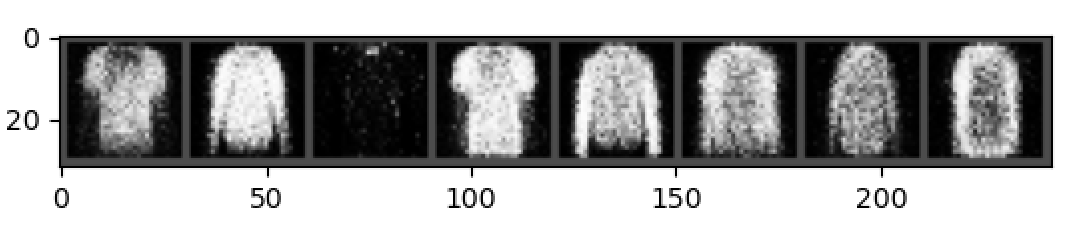
\includegraphics[scale = 0.5]{11.png}\\
   \normalsize{\textbf{训练Loss曲线}}
\end{center}
\begin{center}
   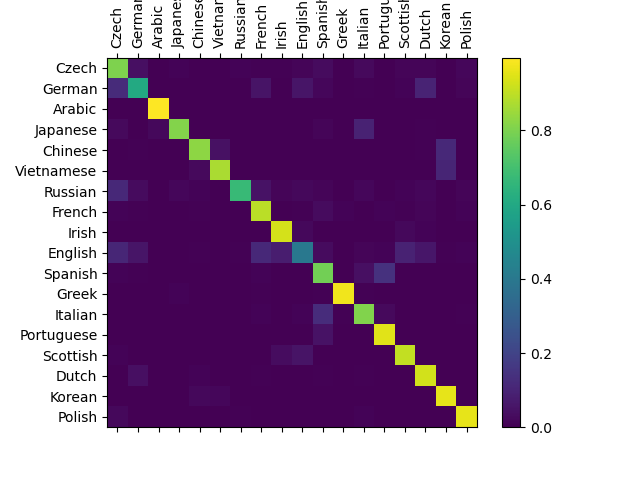
\includegraphics[scale = 0.5]{2.png}\\
   \normalsize{\textbf{准确度曲线图}}
\end{center}
最终,在经历十轮迭代训练后,在验证集上的准确率在96\%左右
\section{个人改进后的MLP}
\subsection{改进后的实验效果}
\subsubsection{epoch = 5}
\begin{center}
   \includegraphics[scale = 0.5]{5_1.png}\\
   \normalsize{\textbf{训练Loss曲线}}
\end{center}
\begin{center}
   \includegraphics[scale = 0.5]{5_2.png}\\
   \normalsize{\textbf{准确度曲线图}}
\end{center}
最终,在经历五轮迭代训练后,在验证集上的准确率在97\%左右
\subsubsection{epoch = 10}
\begin{center}
   \includegraphics[scale = 0.5]{10_1.png}\\
   \normalsize{\textbf{训练Loss曲线}}
\end{center}
\begin{center}
   \includegraphics[scale = 0.5]{10_2.png}\\
   \normalsize{\textbf{准确度曲线图}}
\end{center}
最终,在经历十轮迭代训练后,在验证集上的准确率在98\%左右
\subsubsection{epoch = 20}
\begin{center}
   \includegraphics[scale = 0.5]{20_1.png}\\
   \normalsize{\textbf{训练Loss曲线}}
\end{center}
\begin{center}
   \includegraphics[scale = 0.5]{20_2.png}\\
   \normalsize{\textbf{准确度曲线图}}
\end{center}
最终,在经历二十轮迭代训练后,在验证集上的准确率在98\%左右

\subsection{改进与个人心得}
\subsubsection{网络结构}
我们通过Pycharm软件的python控制台查看运行时的变量,可以看到网络结构如下:
\begin{lstlisting}[language = python]
Net(
  (fc1): Linear(in_features=784, out_features=400, bias=True)
  (fc1_drop): Dropout(p=0.2, inplace=False)
  (fc2): Linear(in_features=400, out_features=80, bias=True)
  (fc2_drop): Dropout(p=0.2, inplace=False)
  (fc3): Linear(in_features=80, out_features=50, bias=True)
  (fc3_drop): Dropout(p=0.2, inplace=False)
  (fc4): Linear(in_features=50, out_features=10, bias=True)
)
\end{lstlisting}
\subsubsection{改进之处和原理}
\begin{itemize}
   \item 首先第一个全连接层的维度由50维改为400维,这样做的原因是因为更大的维度的映射可能可以更好的保存原始图像的特征,带来更好的效果。
   \item 然后下一个全连接层将上一层的400维的数据映射为80维的数据,可以有效的提取重要特征,并对计算量有一定的减小
   \item 接下来在原有的基础上,我又增加了一层全连接层,将上一层处理完的80维的特征映射到50维的线性空间上,再经过这个全连接层将50维的向量映射到10个类别上完成分类。增加的这一层全连接层可以更好地提取每个类别的特点,细化了分类的过程,对提升准确率有着一定的帮助,但同时可能会有过拟合的风险。
   \item 对于训练率我们采用了与原方法相同的0.01,激活函数在测试了Sigmoid型函数效果极其不理想,故更换为原本的RelU函数,通过我们之前学习的知识也可以知道,该激活函数可以更好的拟合非线性的输入和输出特征的映射,比较符合该问题的处理方式。至于动量,由于我们将层数增加,且每层映射的线性空间增大,故将其设置为0.8。每一层之间的drop\_out随机丢弃率仍然为0.2,损失函数仍然是交叉熵函数。
   \item 随后我又用卷积的方法进行了测试,因为图片本身是二维向量,二维处理的效果应该是优于一维的,而实际经过测试,经过两层卷积和一层隐层的效果可以轻松达到98\%,只是训练时间较长,训练数据量较大。
\end{itemize}
\subsubsection{实验心得}
通过这次实验,我对Pytorch的使用有了深入的理解。首先是torch.nn模块,该模块定义好了各个神经层的结构(如卷积层、全连接层等),可以直接调用使用,torch.nn.functional中定义了常见的函数等,torch.utils.data.DataLoader则是对数据集进行细分的处理。总体来说,只要设计出了网络结构,那么搭建网络换个训练的过程就像是搭积木一样,一层层调用即可。对于MLP经网络,我更好的了解了张量在每一层之间的向下传递过程,以及在训练时通过损失函数向前反馈,通过求导进行计算梯度进行梯度下降更新参数的过程,对深度学习有了更好的认识。
\end{document}